\documentclass[12pt]{article}
\usepackage[utf8]{inputenc}
\usepackage{graphicx}
\graphicspath{ {./images/} }

\title{Introduction to Computer Science\\ Project report}
\author{Ding Yi Zhang
\and David Alexander}
\date{22 May 2019}

\begin{document}

\maketitle


\section{Introduction}
Binary star systems consist of two stars that orbit each other. Here on Earth, we only have one Sun, but in a binary system, there would be two nearby stars, like on Tatooine in Star Wars. These star systems are surprisingly common, and the nearest solar system to ours, the Centauri system, is made up of a binary star system and another orbiting star. Stars are quite easy to detect using modern astronomical methods. Planets, however, being much smaller and much less bright, are more difficult to spot. Therefore, the question that our term project aims to answer is: what would the orbit of a planet orbiting a binary system look like? This is an applied version of the three-body problem, but it is also a relevant scientific question. Given how common these systems are, it would be interesting to see how a possibly habitable planet would orbit around a system like Centauri. And more importantly; would Luke really be able to see two sunsets at once?

\section{Scientific Basis}
Astronomy is a very ancient field, and many of the equations that we will use were discovered as far back as the 17th Century, by a man named Johannes Kepler. He theorized three laws, now known as Kepler’s laws. The first law states that any body orbiting another body will follow a path in the shape of an ellipse. For example, Earth’s orbit around the Sun, which appears circular, is in fact a near perfect ellipse. Ellipses have a major and a minor axis, the major axis being longer than the minor, and contain two focus points. Kepler’s first law also states that the orbited body will be at one of the two focus points. Kepler’s second law describes the velocities of the two bodies. It states that areal velocity, or $m^2/s$, stays constant as long as there is no tangential acceleration. This means that the angular and tangential velocities of an orbiting body will depend on how far it is from the focus: the further it is, the slower it will go, and the closer it is, the faster it will go. From this law we can derive equations to find the velocity of an object at any given point on its orbit. The third law states that there is a relation between the mass of the two bodies, the semi-major axis of the orbit and the period of the orbit, and that for the same conditions, the exact same orbit will be obtained. All these laws can also be related back to and derived from a single equation; Newton’s law of universal gravity, and binary systems also obey these laws. Therefore if we have the mass and initial positions of the two stars, we can simulate the binary system.

As previously mentioned, planets are much more difficult to detect than stars. The vast majority of these have been detected using the transit method and the radial velocity method. The former uses periodic dips in the luminosity received from a star to infer the presence of a planet passing in front of it, and measuring its velocity, which can be used along with its orbital period and Kepler's second and third laws to determine how far from the star it is. The radial velocity measures tiny Doppler shifts in the spectral signature of a star to measure the tiny changes in the velocity of the star caused by the planet's gravity. This can then be used to find the planet's mass. While these values can give provide us with some information about the planet, they do not provide much information about the orbital path of the planet, especially relative to the other bodies in the system. They are, however, the required initial conditions for our model, which shows the orbital path of these bodies.

\section{Mathematical Models}
All three of Kepler’s laws can be related back to and derived from a single equation; Newton’s universal law of gravity. This law is what makes the others true. Newton’s law simply gives the gravitational force, and therefore acceleration, felt by one object due to another. This means that with the right initial conditions, we can simulate the entire system using only universal gravity and kinematics equations; Kepler’s laws should hold, since they are based on universal gravity. The problem then becomes one of numerical integration, and calculating the acceleration,velocity and position of each object involved after a certain small timestep. For this we will use a modified, self-starting version of Verlet’s method: \[x_{n+1} = x_{n} + v_{n}dt + \frac{1}{2}a_{n}(dt)^{2}\]
\[v_{n+1} = v_{n} + \frac{1}{2}(a_{n+1} + a_{n})dt\]
This simplifies our code, as we don’t have to worry about calculating an initial step or two with a different method. This method starts with an initial position and velocity. It calculates initial acceleration using initial position, and calculates the next position using initial velocity, acceleration and position. Using this new position, it recalculates acceleration, and then using the new acceleration and the previous acceleration, and finds the new velocity. Then it calculates the next position, and so on. The precision of our simulation depends on the size of our timestep, and is accurate to the fourth derivative of position.

\section{Verification and results}
To verify the accuracy of our model, we simulated the Earth-Moon-Sun system and measure the period of the Moon's orbit around Earth. 
\begin{figure}[ht]
    \centering
    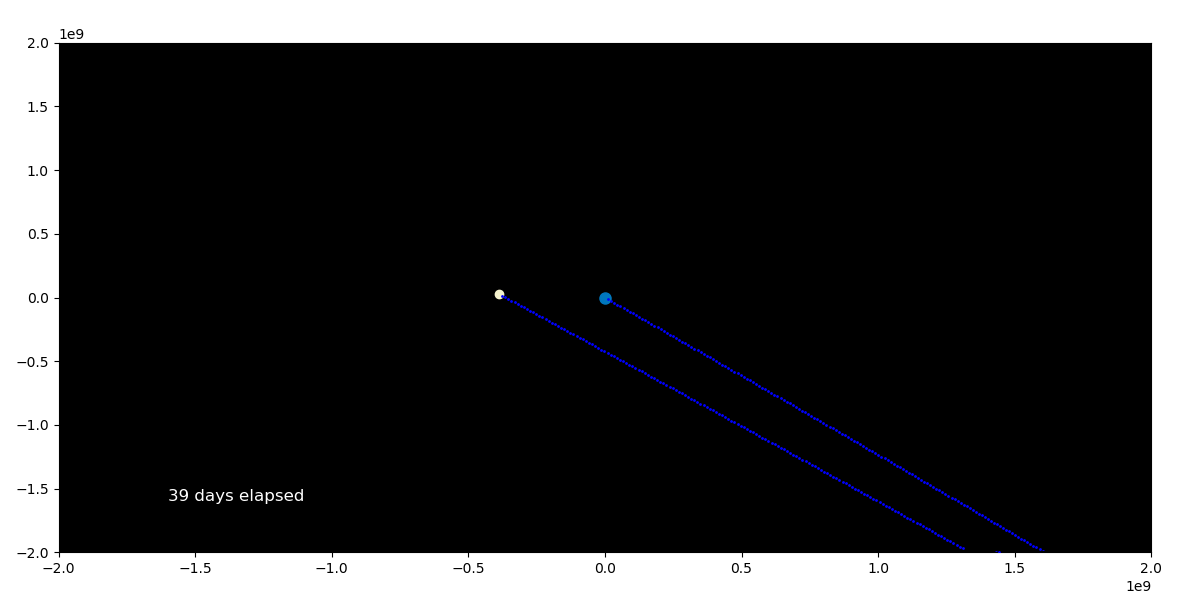
\includegraphics[width=\textwidth]{sem}
    \caption{The Moon orbiting the Earth}
\end{figure}
The average period in our simulation, defined as the time from one full moon to the next, was calculated to be 29.52 days. The real measured value is approximately 29.53 days. This gives us an error of less than 0.035\%, and we can therefore conclude that our model is accurate.

The system we studied with our model was one of our own creation. 


\end{document}
